\uuid{AIFJ}
\exo7id{6925}
\titre{exo7 6925}
\auteur{ruette}
\organisation{exo7}
\datecreate{2013-01-24}
\isIndication{false}
\isCorrection{true}
\chapitre{Probabilité continue}
\sousChapitre{Densité de probabilité}

\contenu{
\texte{
\def\I1{{ \rm 1\:\!\!\! l}}
Soit $X$ et $Y$ des variables aléatoires indépendantes de loi uniforme 
de densité $\I1_{[0,1]}$
et $Z=X+Y$. Calculer la loi de $Z$.
}
\reponse{
\def\I1{{ \rm 1\:\!\!\! l}}
On donne 2 méthodes graphiques et un calcul direct.

On peut prendre comme modèle $\Omega=[0,1]^2$, $P$ la mesure de 
Lebesgue sur le carré, $X(x,y)=x$, $Y(x,y)=y$. On peut alors 
représenter $Z=t$ par la droite d'équation $x+y=t$ dans le carré (figure
de gauche).

Si $0\leq t\leq 1$ alors $F_Z(t)=P(X+Y\leq t)=\frac{t^2}{2}$ (figure
de gauche).
Si $1\leq t\leq 2$, alors $F_Z(t)=1-\frac{(2-t)^2}{2}$ (figure du milieu).
Si $t<0$ alors $F_Z(t)=0$ et si $t>2$ alors $F_Z(t)=1$.

$F_Z$ est continue sur $\Rr$, $C^1$ par morceaux, on peut donc dériver
pour obtenir $f_Z$ la densité de $Z$ : $f_Z(t)=t$ si $0\leq t\leq 1$,
$f_Z(t)=2-t$ si $1\leq t\leq 2$, $f_Z(t)=0$ sinon.

\medskip
On peut également calculer la densité directement, ``à la
physicienne'', en considérant $dt$ comme un tout petit accroissement
(on l'a dessiné assez gros pour rendre le dessin lisible). 
Sur la figure de droite,
on a dessiné $X+Y\in [t,t+dt]$ pour $0\leq t\leq 1$. L'aire de la
partie hachurée est à peu près $t\sqrt{2}\times\frac{dt}{\sqrt{2}}$ (longueur
$\times$ largeur), donc on  a $P(t\leq X+Y\leq t+dt)=tdt$. Or
$P(t\leq Z\leq t+dt)=f_Z(t)dt$, ce qui donne la
densité $f_Z(t)=t$ pour $0\leq t\leq 1$. On fait pareil pour $1\leq t\leq 2$.

%\bigskip
\centerline{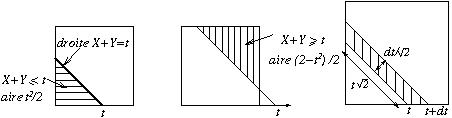
\includegraphics{../images/img006925-1}}
%\vspace{1cm}

\medskip
Calcul direct : La densité de $X$ et $Y$ est $f(t)=\I1_{[0,1]}(t)$. Par
indépendance, $Z=X+Y$ a une densité $f_Z(t)=f*f(t)=\displaystyle
\int_{\Rr} f(t-x)f(x)dx$ (résultat du cours, qu'on peut redémontrer
par changement de variable à partir de la définition de $P_X*P_Y$).

$f(t-x)f(x)=1$ si $0\leq t-x\leq 1$ et $0\leq x\leq 1$,
$f(t-x)f(x)=0$ sinon.

Soit $D_t=\{x\in\Rr\mid 0\leq t-x\leq 1 \mbox{ et } 0\leq x\leq 1\}=
\{x\in\Rr\mid  t-1\leq x\leq t\mbox{ et }0\leq x\leq 1\}$. $D_t=
[\max (0,t-1),\min(t,1)]$. On a
$f_Z(t)=\displaystyle\int_{D_t} 1 \, dx$, alors :\\
-- si $0\leq t\leq 1$, $D_t=[0,t]$ et $f_Z(t)=t$,\\
-- si $1\leq t\leq 2$, $D_t=[t-1,1]$ et $f_Z(t)=2-t$,\\
-- si $t<0$ ou $t>2$, $D_t=\emptyset$ et $f_Z(t)=0$.
}
}
